\documentclass{article} % kind of document
\usepackage[utf8]{inputenc} %encoding of choice
\usepackage[american]{babel} %language of choice
\usepackage[p,osf]{cochineal}
\usepackage{fancyhdr} %for header
\usepackage{amsmath, tabu} %math mode
\usepackage{mathtools}
\usepackage{amssymb} %math symbols
\usepackage{dsfont} %specifically for the indicator function symbol
\usepackage{xcolor} %to color text
\usepackage{amsthm} %math theorem
\usepackage{tikz}
\usepackage{subcaption}
\usepackage{caption}
\usepackage{multirow}
\usepackage[bottom]{footmisc}
\usepackage[colorlinks=true, citecolor=blue, linkcolor=blue, urlcolor=blue]{hyperref} %to create hyperlinks
% \usepackage[dvipsnames]{xcolor}
\usepackage{enumerate} %make lists
\usepackage{graphicx} %insert images
\usepackage{float} %to fix image position
\usepackage{moreverb} %to make boxes
\usepackage{lipsum} %lorem ipsum package
\usepackage{setspace} % to use singlespace below in the solution environment
\usepackage[shortlabels]{enumitem}
\usepackage{parskip}
\usepackage[us]{datetime} %package for setting due date in US format
\newdate{duedate}{29}{09}{2021} %to set a due date
% \usepackage{jlcode}
\allowdisplaybreaks
\usepackage[margin=1in]{geometry}
\pagestyle{fancy}
\usepackage{jlcode}

\lhead{Due: \displaydate{duedate}}
\chead{ECON 899 -- Problem Set 4}
\rhead{Danny, Mitchell, Ryan, Yobin, and Hiroaki}
\title{ECON 899 -- Problem Set 4}
\author{Danny, Mitchell, Ryan, Yobin, and Hiroaki}
\date{\today}

\DeclareMathOperator*{\E}{\mathbb{E}} %ease of writing e and E
\newcommand{\e}{\mathrm{e}}
\newcommand{\ct}{\mathsf{c}}
\newcommand{\Z}{\mathbb{Z}}
\newcommand{\R}{\mathbb{R}}
\newcommand{\N}{\mathbb{N}}
\newcommand{\ifn}{\mathds{1}}
\newcommand{\X}{\mathbf{X}}
\newcommand{\Y}{\mathbf{Y}}
\newcommand{\one}{\mathbf{1}}
\newcommand\numberthis{\addtocounter{equation}{1}\tag{\theequation}}
\newcommand*\widebar[1]{\overline{#1}} % to get a widebar
\theoremstyle{definition}
\newtheorem{theorem}{theorem} % Theorem display format
\newtheorem{problem}[theorem]{Exercise} % Problem display format, last bracket sets display choice

\newenvironment{solution}[1][Answer]{\begin{singlespace}\underline{\textbf{#1:}}\quad }{\ \rule{0.3em}{0.3em}\end{singlespace}} % Answer format

\newenvironment{solutions}[1][Proof]{\begin{singlespace}\underline{\textbf{#1:}}\quad }{\ \rule{0.3em}{0.3em}\end{singlespace}} % Answer format

\begin{document}
\maketitle
\subsubsection*{Exercise 1}
\begin{enumerate}
\item  Use the parametrization from the previous problem set. We continue to assume that labor supply is endogenous. Solve for the stationary equilibrium with social security $ (\theta^{SS}_0 = 0.11) $ and without it $ (\theta^{SS}_N = 0) $ following the algorithm described in the lecture notes (\textit{Step 1: Calculating the stationary competitive equilibrium}). Denote the initial distribution of agents over age, $ j $, asset holdings, $ a $, and productivity levels, $ z $, by $  \Gamma_0^{SS}(z,a,j;\theta_0^{SS}) $. Denote the welfare of agents alive in the initial steady state by $ V_0^{SS}(z,aj;\theta_0^{SS})$.
  
\item  Compute the transition path of the economy using the algorithm in \textit{Step 2: Solving for the transition path} in the lecture notes. Try N = 30 for the
  number of periods it approximately takes to get to the new steady state. Obtain and store the value function for the generations in the initial steady state, $ V_0(z,a,j; \theta_0^{SS}, \theta_N^{SS}) $. Plot the transition paths of interest rate, wage, capital and effective labor. Comment on the results you obtain.
  \begin{solution}
    During the transition dynamics, capital adjusts gradually. Efficient labor supply jumps in the policy period, which induces jumps in the interest rate and wage at the beginning. Afterward, all variables smoothly transit to the new steady state. Figure \ref{fig} contains the results.
    \begin{figure*}
      \centering
      \begin{subfigure}[b]{0.475\textwidth}
        \centering
        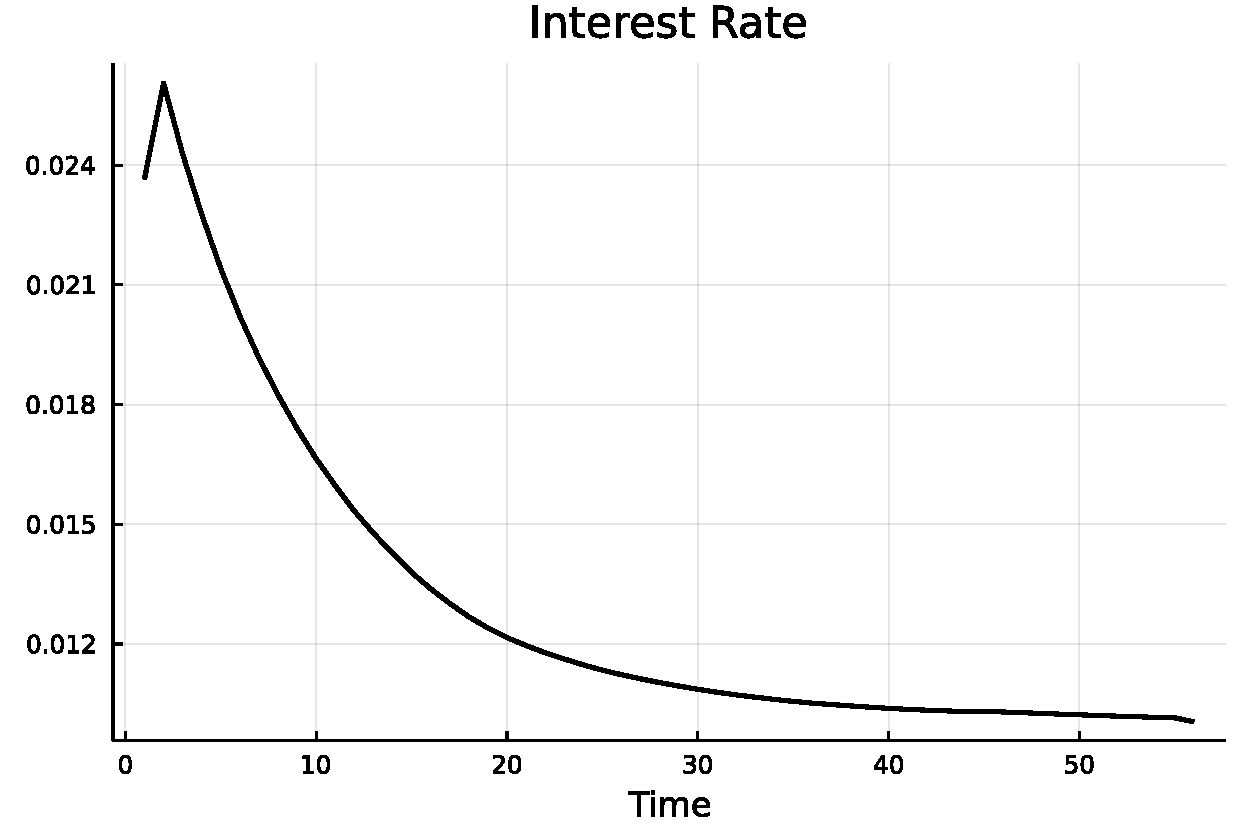
\includegraphics[width=\textwidth]{Figures/interest_rate.pdf}
      \end{subfigure}
      \hfill
      \begin{subfigure}[b]{0.475\textwidth}  
        \centering 
        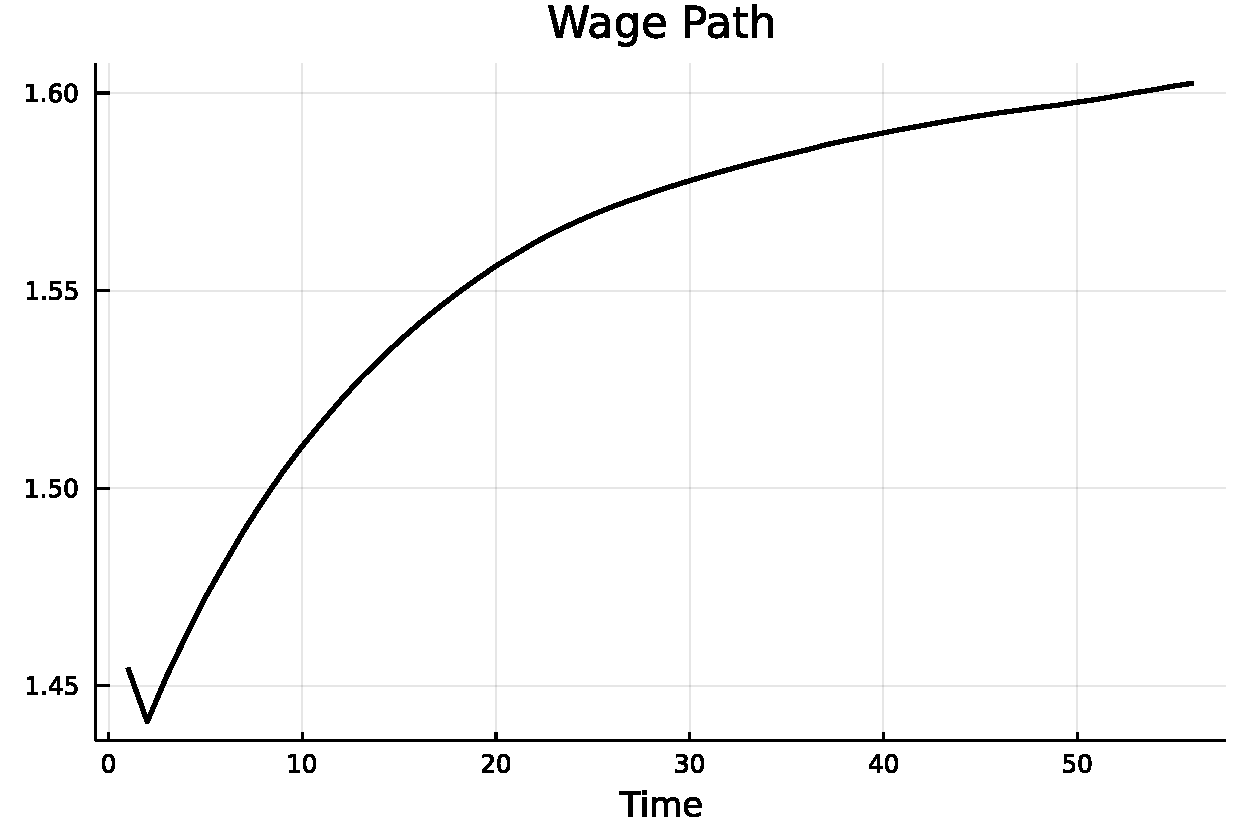
\includegraphics[width=\textwidth]{Figures/wage.pdf}
      \end{subfigure}
      \vskip\baselineskip
      \begin{subfigure}[b]{0.475\textwidth}   
        \centering 
        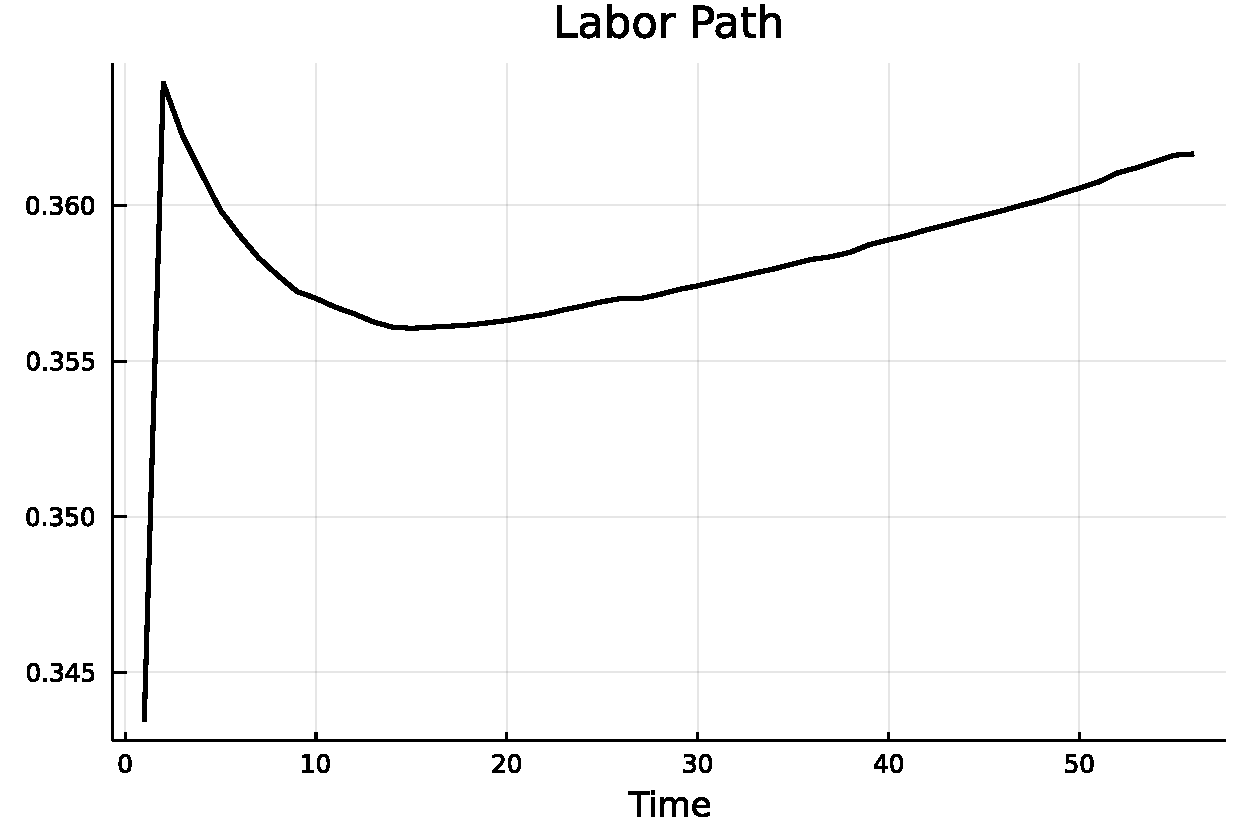
\includegraphics[width=\textwidth]{Figures/labor.pdf}
      \end{subfigure}
      \hfill
      \begin{subfigure}[b]{0.475\textwidth}   
        \centering 
        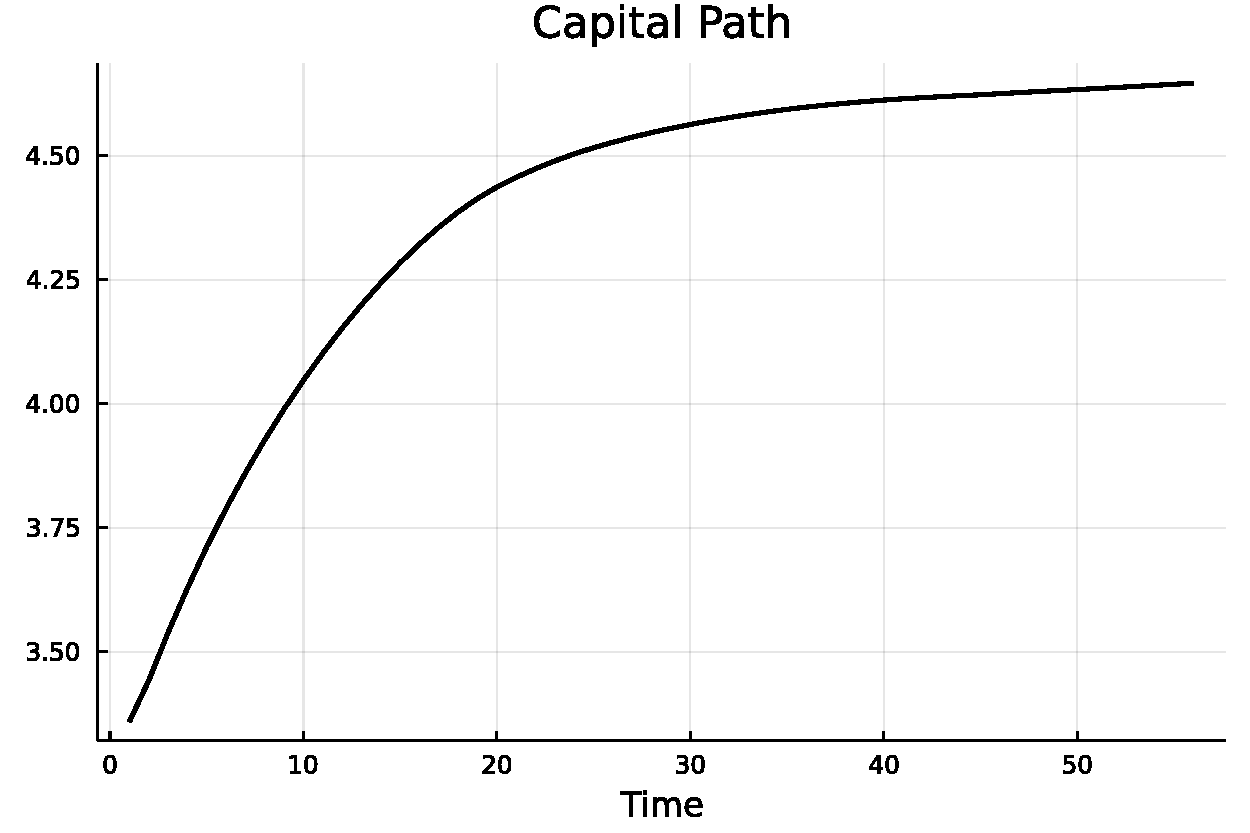
\includegraphics[width=\textwidth]{Figures/capital.pdf}
      \end{subfigure}
      \caption{Transition Path: Unanticipated Shock}
      \label{fig}
    \end{figure*}
  \end{solution}
  
\clearpage  
\item  What fraction of the overall population would support the reform? Compute and plot the measure of consumption equivalent variation for each age, $ EV_j $ , using $$ EV_j = \sum_z \int_a EV(z,a,j)  \Gamma_0^{SS}(z,a,j; \theta_0^{SS})  da, $$ with \[  EV(z,a,j) = \left(  \frac{ V_0(z,a,j; \theta_0^{SS}, \theta_N^{SS}) }{  V_0^{SS}(z,a,j; \theta_0^{SS}) } \right)^{\frac{1}{\gamma(1 - \sigma)}} . \] Discuss the results.		
  \begin{solution}
	
    All age groups prefer policy with social security, but younger generations dislike it the least. Figure \ref{EV1} shows the results.

\begin{figure}[htbp]
    \begin{center}
      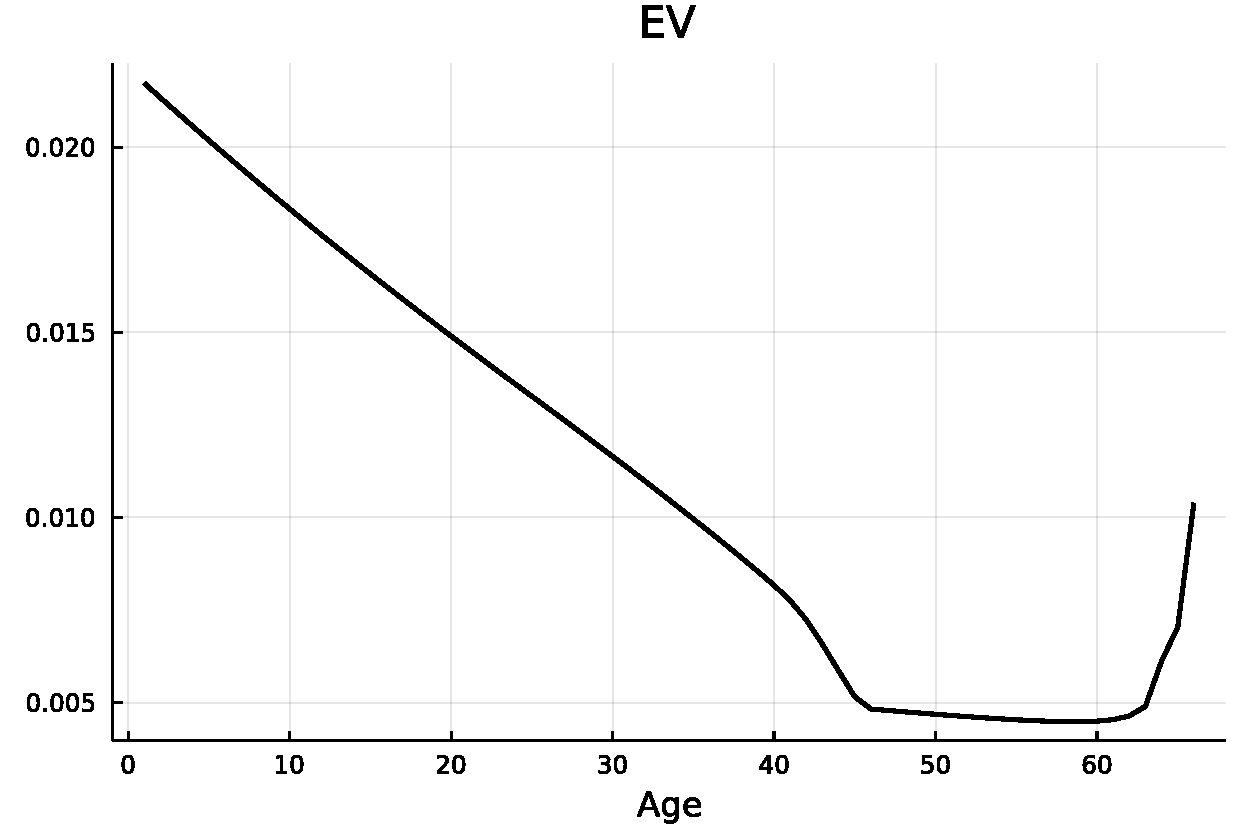
\includegraphics[width=0.5\textwidth]{Figures/EV.pdf}
	\caption{Consumption Equivalent Variation}
      \label{EV1}
    \end{center}
\end{figure}
    
  \end{solution}
\end{enumerate}


\subsubsection*{Exercise 2}
\begin{enumerate}
\item Instead of considering an unexpected elimination of the social security system, assume that in $ t = 0 $ the government credibly announces that it is going to abolish the public pension system starting from $ t = 21 $ onwards. Thus, all individuals retired keep their social security benefits, but future retirees anticipate that they will receive only part or no social security benefits. Repeat steps (1)-(3) of exercise 1 to study how agents readjust their plans and how political support changes for the anticipated reform in 21 years. You will have to increase the number of transition periods (try $ N = 50 $). Discuss your results.
  \begin{solution}
    With an expected policy change, agents start to adjust from the announcement period, while they also make a relatively bidder adjustment when the policy change happens, especially for labor supply. But capital adjustment is smoother, and most of the adjustment happens before policy changes.
    With an expected policy change, the welfare loss is lower. Figures \ref{fig2} and \ref{EV2} display the results.
    \begin{figure*}
      \centering
      \begin{subfigure}[b]{0.475\textwidth}
        \centering
        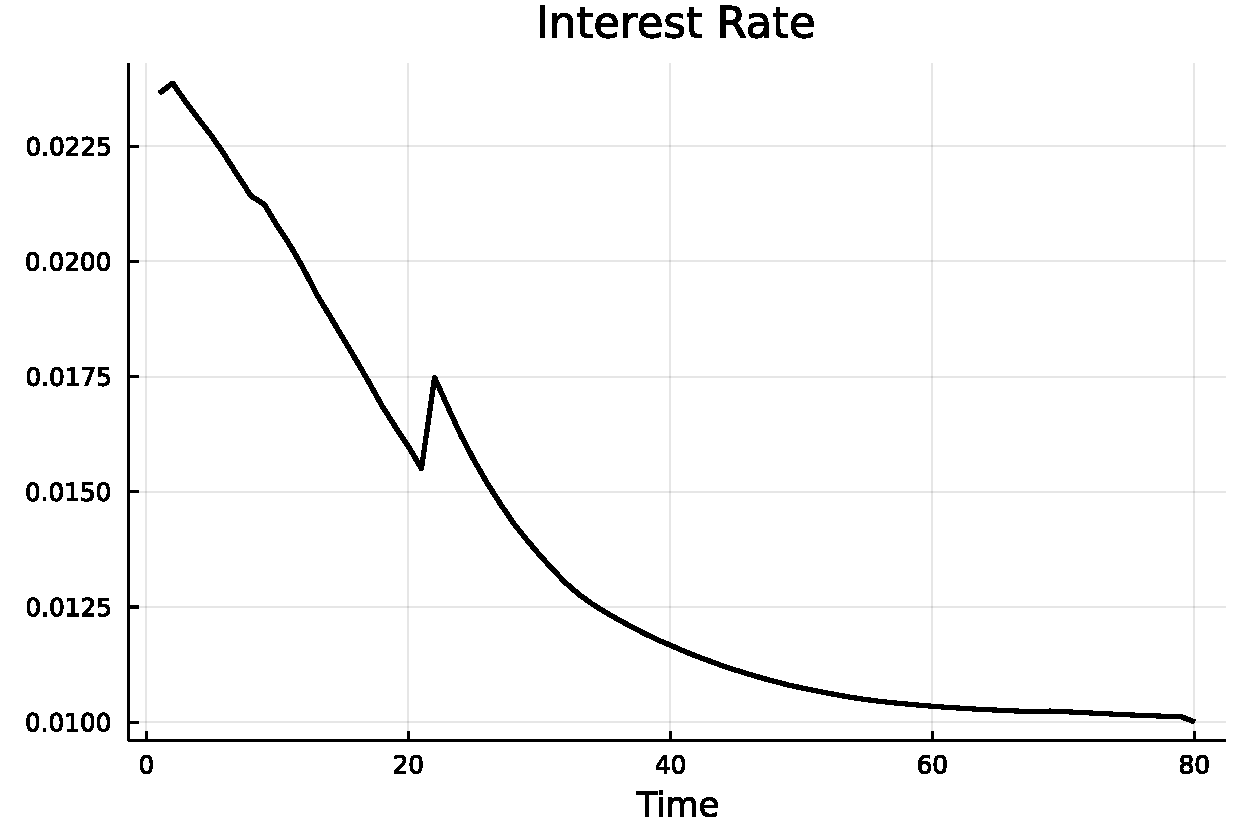
\includegraphics[width=\textwidth]{Figures/interest_rate_ex2.pdf}
      \end{subfigure}
      \hfill
      \begin{subfigure}[b]{0.475\textwidth}  
        \centering 
        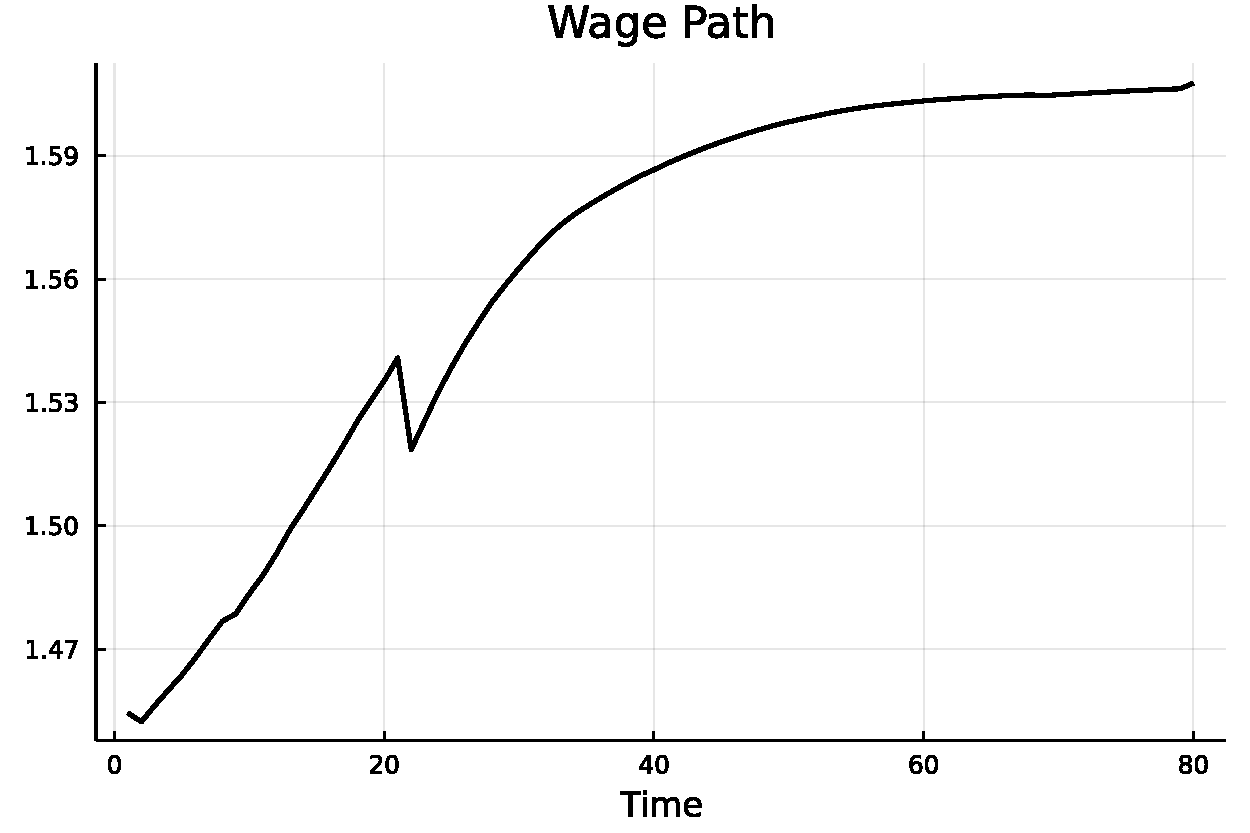
\includegraphics[width=\textwidth]{Figures/wage_ex2.pdf}
      \end{subfigure}
      \vskip\baselineskip
      \begin{subfigure}[b]{0.475\textwidth}   
        \centering 
        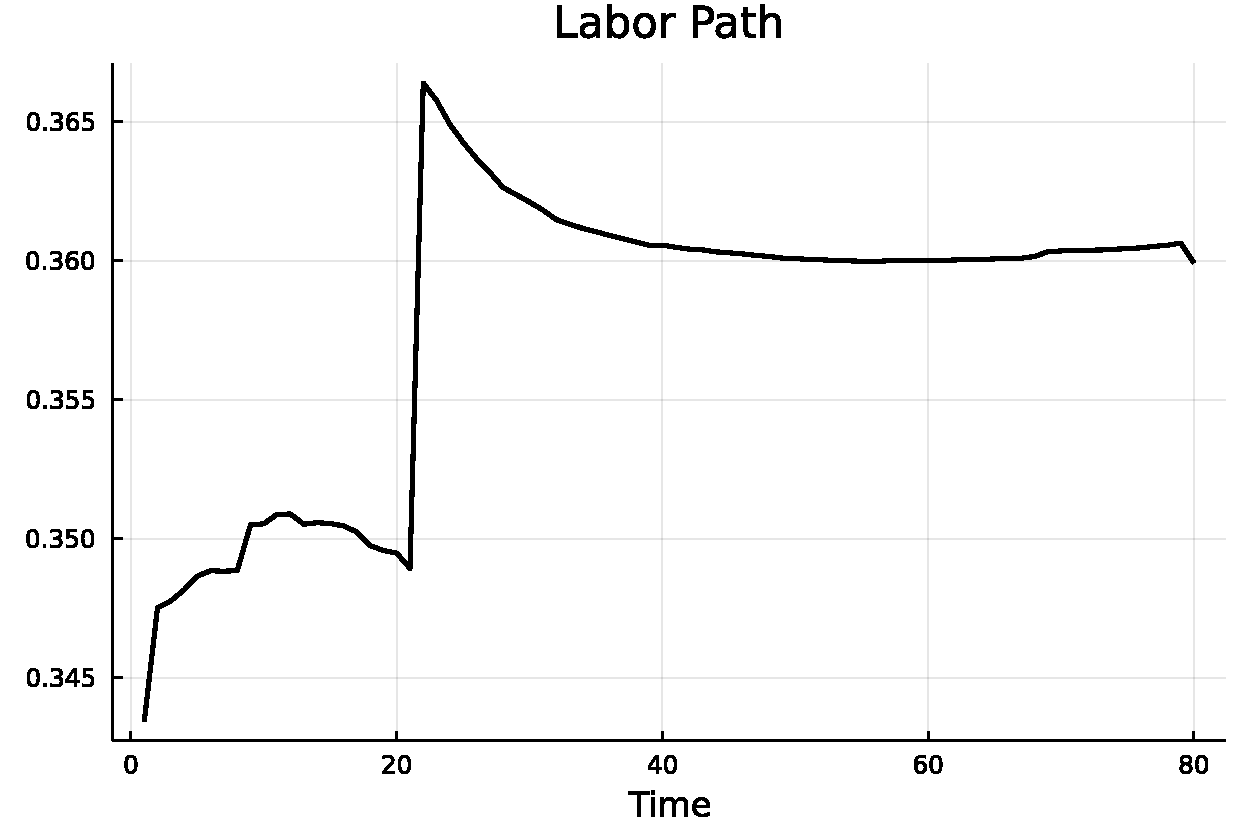
\includegraphics[width=\textwidth]{Figures/labor_ex2.pdf}
      \end{subfigure}
      \hfill
      \begin{subfigure}[b]{0.475\textwidth}   
        \centering 
        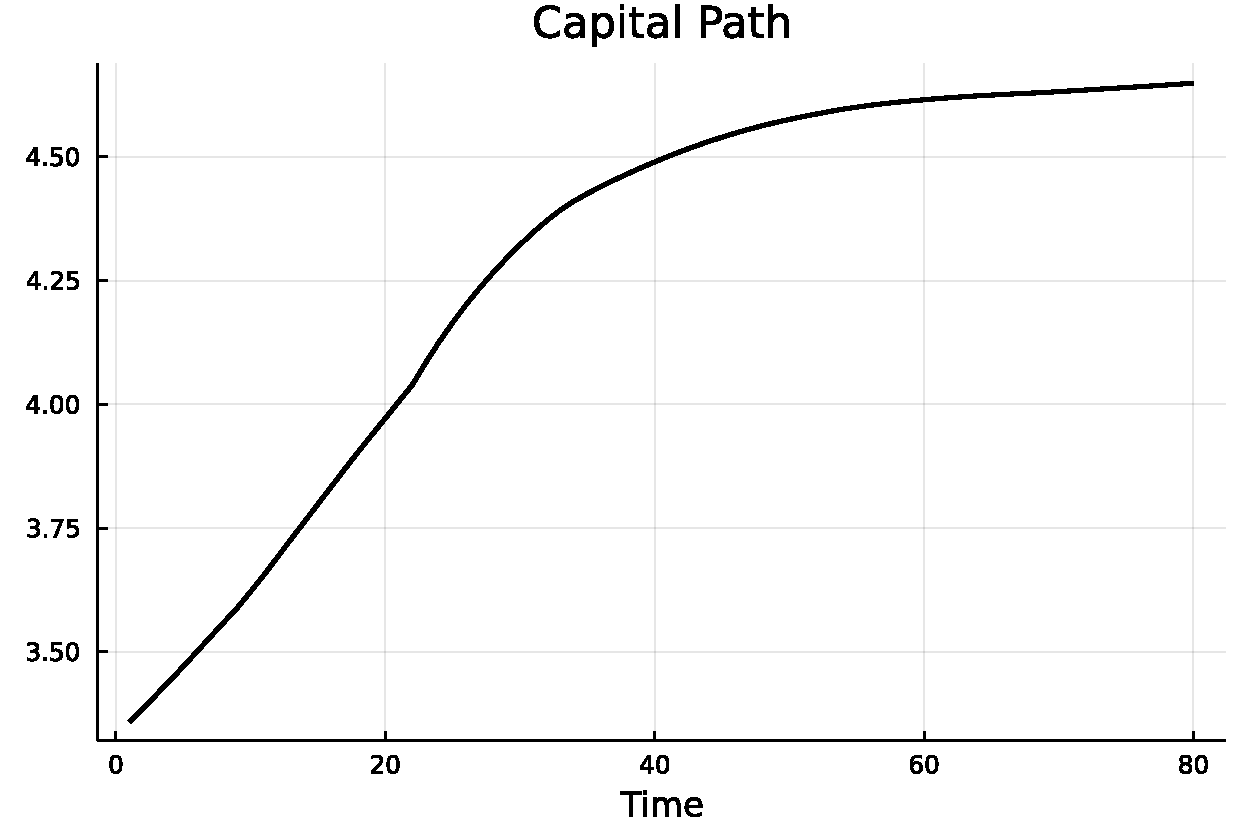
\includegraphics[width=\textwidth]{Figures/capital_ex2.pdf}
      \end{subfigure}
      \caption{Transition Path: Anticipated Shock}
      \label{fig2}
    \end{figure*}
    \clearpage
	\begin{figure}
	    \begin{center}
	      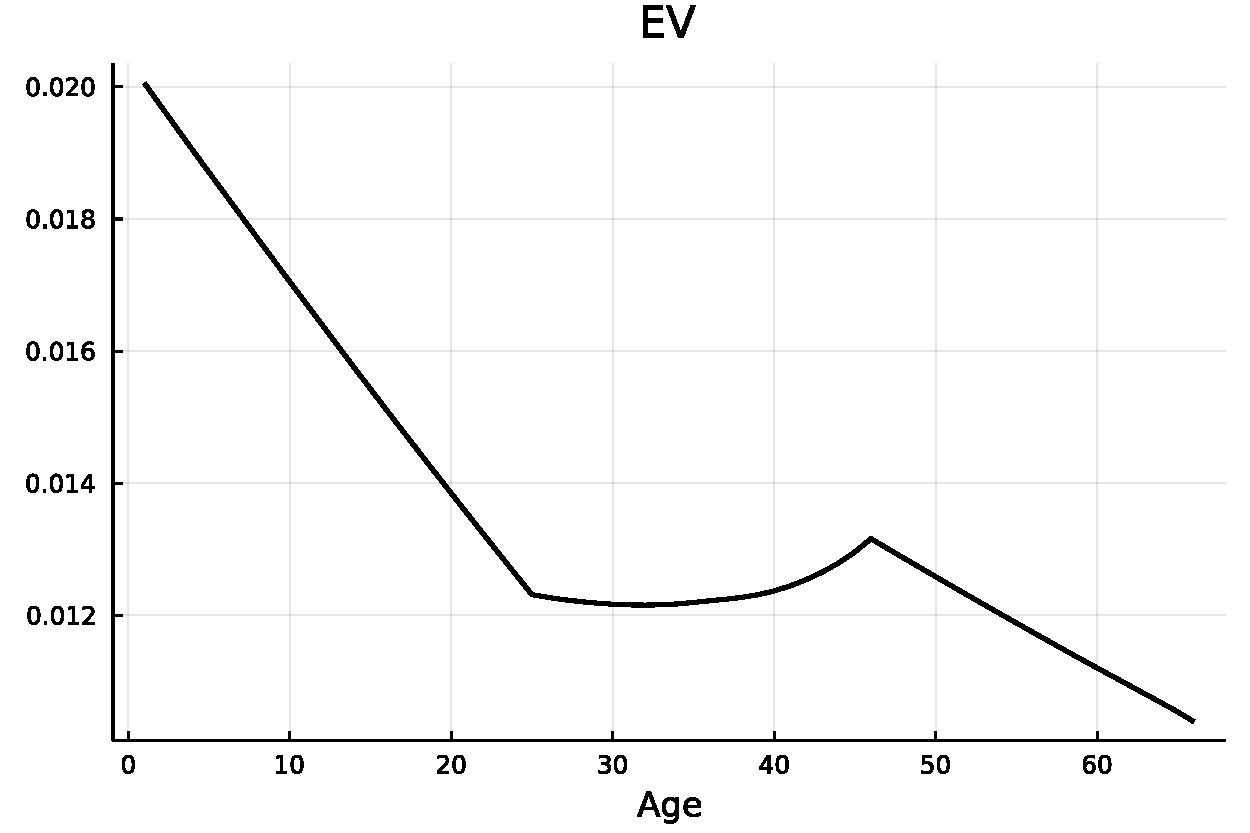
\includegraphics[width=0.5\textwidth]{Figures/EV_ex2.pdf}
		\caption{Consumption Equivalent Variation for Exercise 2}
		\label{EV2}
	    \end{center}
	\end{figure}
  \end{solution}
\end{enumerate}
\newpage
	\section*{Appendix}
 	The first code file runs the code.
 	\jlinputlisting{Code/run_model.jl}
	
 	The second code file contains the relevant functions.
 	\jlinputlisting{Code/conesa_kueger.jl}
\end{document}